\chapter{Classificazione} %\label{3cap:classificazione}

\begin{preamble}
{\em In questo capitolo viene affrontato il problema della classificazione, una tecnica di apprendimento supervisionato che consente di assegnare i dati a categorie predefinite sulla base delle loro caratteristiche. Tale approccio viene applicato al contesto dei mercati energetici per individuare diverse condizioni di prezzo e di funzionamento del sistema elettrico.}
\end{preamble}


La classificazione è una tecnica di apprendimento supervisionato che consente di assegnare i dati a categorie predefinite. Nel seguente studio sono stati condotti quattro diversi task, tutti basati sul prezzo orario \textit{day-ahead} (\texttt{price}, in €/MWh) e sul mix di produzione delle zone di mercato, di seguito elencati:
\begin{itemize}
    \item \textbf{T1 -- Classificare le ore a prezzo nullo o negativo}\\
    Stabilire se il prezzo orario di una zona di mercato è minore o uguale a zero, a partire dalla produzione per fonte, dall'ora del giorno, dal giorno della settimana e dalla zona.
    \item \textbf{T2 -- Classificare l'ora rispetto al prezzo medio giornaliero}\\
    Determinare se il prezzo di una determinata ora è superiore o inferiore al prezzo medio della stessa zona nello stesso giorno.
    \item \textbf{T3 -- Classificare il prezzo in base alla fascia di prezzo della zona}\\
    Assegnare ciascuna ora a una delle quattro fasce di prezzo (bassa, medio-bassa, medio-alta, alta), definite dai quartili del prezzo di ogni zona nell'anno 2024.
    \item \textbf{T4 -- Classificare la fascia oraria della giornata}\\
    Identificare la fascia del giorno (notte, mattina, pomeriggio, sera) a partire dal mix di produzione, senza utilizzare l'ora tra le variabili di input.
\end{itemize}
Questo capitolo descrive in dettaglio i passi intrapresi, partendo dalla preparazione dei dati e dalla validazione temporale (addestramento sul 2024 e test da gennaio a giugno 2025) fino all'analisi comparativa dei modelli, evidenziando le principali sfide affrontate, tra cui lo sbilanciamento delle classi e lo spostamento di distribuzione dei prezzi tra i due periodi, e i risultati ottenuti.

\section{Task 1: Classificazione dei Prezzi Nulli o Negativi}
\label{sec:task1_descrizione}

\subsection{Definizione dell'Obiettivo}
Il primo task predittivo \textbf{Task 1 (T1)}, consiste nella classificazione binaria delle ore in cui il prezzo dell'energia elettrica sul mercato all'ingrosso subisce un crollo, raggiungendo valori nulli o negativi. 

Dal punto di vista dell'ingegneria dei mercati energetici, i prezzi negativi rappresentano un'anomalia sistemica di grande interesse. Essi si verificano tipicamente quando vi è una forte rigidità al ribasso della generazione tradizionale (ad esempio, impianti nucleari o a carbone che non possono essere spenti rapidamente) unita a un picco improvviso e non programmato di generazione da fonti rinnovabili non programmabili (fotovoltaico ed eolico), in momenti di bassa richiesta. Riuscire a prevedere con precisione tali eventi fornisce un vantaggio strategico fondamentale per i produttori dell'energia.

Matematicamente, il task è stato formalizzato creando una variabile target binaria $Y_{T1}$, derivata direttamente dal prezzo orario del mercato ($P_{h}$), secondo la seguente regola logica:

\begin{equation}
Y_{T1} = 
\begin{cases} 
1, & \text{se } P_{h} \leq 0 \text{ \euro / MWh} \\
0, & \text{se } P_{h} > 0 \text{ \euro / MWh}
\end{cases}
\end{equation}

\subsection{Criticità del Dataset: Sbilanciamento delle Classi e Anomaly Detection}
\label{subsec:t1_sbilanciamento}
La caratteristica fondante del Task 1 è il forte sbilanciamento delle classi in esame. Su un dataset netto di 288.288 osservazioni orarie, distribuite su 22 zone di mercato europee, le istanze in cui si è verificato un prezzo nullo o negativo ammontano a sole 14.070 unità. 

La distribuzione del target risulta pertanto la seguente:
\begin{itemize}
    \item \textbf{Classe 0 (Prezzo Positivo):} $\sim 95.2\%$ del dataset (classe maggioritaria).
    \item \textbf{Classe 1 (Prezzo $\leq$ 0):} $\sim 4.8\%$ del dataset (classe minoritaria).
\end{itemize}

Questa sproporzione inquadra il problema all'interno del dominio dell'\textit{Anomaly Detection}. 

\subsection{Metriche di Valutazione Scelte}
Per ovviare al problema dell'accuratezza globale, l'addestramento e l'ottimizzazione degli algoritmi per il Task 1 sono stati guidati massimizzando le seguenti metriche sulla classe minoritaria (Classe 1):

\begin{itemize}
    \item \textbf{Recall (Sensibilità):} Rappresenta la percentuale di veri crolli di prezzo correttamente individuati dal modello rispetto al totale dei crolli reali. Nel contesto energetico, massimizzare la Recall è l'obiettivo primario, poiché il "mancato allarme" (non prevedere un prezzo zero imminente) comporta ingenti perdite economiche.
    \item \textbf{Precision (Valore Predittivo Positivo):} Misura l'affidabilità del modello quando prevede un'anomalia. Un'alta Precision riduce i "falsi allarmi", ovvero le situazioni in cui il modello prevede un calo di prezzo che non si verifica.
    \item \textbf{F1-Score:} Media armonica tra Precision e Recall, utilizzata come indicatore sintetico per valutare la robustezza e l'equilibrio complessivo del classificatore sulla classe critica.
\end{itemize}

Sulla base di queste premesse, nella sezione successiva si procederà al confronto delle prestazioni di cinque diversi algoritmi di Machine Learning (Random Forest, K-Nearest Neighbors, Decision Tree, Naive Bayes e Gradient Boosting), analizzandone il comportamento di fronte allo sbilanciamento strutturale dei dati.

\subsection{Preparazione dei Dati}
\label{subsec:t1_prep_dati}

Prima di procedere all'addestramento dei modelli di \textit{Machine Learning}, è stata effettuata un'accurata fase di definizione delle variabili (\textit{Feature}) e di partizionamento del dataset.

Per l'addestramento dei classificatori è stata definita una matrice di input basata sulle seguenti feature:
\begin{itemize}
    \item \textbf{Produzione energetica (MW):} \texttt{solar}, \texttt{wind\_onshore}, \texttt{wind\_offshore}, \texttt{nuclear}, \texttt{fossil\_gas}, \texttt{fossil\_hard\_coal}, \texttt{fossil\_brown\_coal\_lignite}, \texttt{hydro\_total}, \texttt{biomass}, \texttt{waste}.
    \item \textbf{Variabili temporali:} \texttt{ora} (0–23) e \texttt{giorno\_settimana} (0–6).
    \item \textbf{Variabile spaziale:} \texttt{country} (codificata tramite One-Hot Encoding con \textit{drop\_first}).
\end{itemize}

Al fine di garantire una valutazione rigorosa e prevenire il fenomeno del \textit{data leakage} (interferenza di informazioni future nell'addestramento), il dataset non è stato suddiviso casualmente, ma è stato applicato un \textbf{partizionamento temporale (Out-of-Time Validation)}. Lo split è stato fissato al $1^{\circ}$ gennaio 2025:
\begin{itemize}
    \item \textbf{Training Set (storico 2024):} impiegato per l'addestramento dei modelli e l'apprendimento dei pattern sulle dinamiche di mercato del primo anno.
    \item \textbf{Test Set (dati futuri 2025):} set di validazione isolato, utilizzato esclusivamente in fase di inferenza per simulare la reale capacità predittiva del modello su un orizzonte temporale nuovo e non ancora osservato.
\end{itemize}

\section{T1: Random Forest}

Utilizzando l'algoritmo di ML \textit{Random Forest} si hanno i seguenti Risultati:

\begin{table}[htbp]
    \centering
    \caption{Report di classificazione del Random Forest (Task 1)}
    \label{tab:report_rf_task1}
    \begin{tabular}{|l|c|c|c|c|}
        \hline
        \textbf{Classe} & \textbf{Precision} & \textbf{Recall} & \textbf{F1-Score} & \textbf{Supporto} \\ \hline
        Prezzo $>$ 0    & 0.98 & 0.94 & 0.96 & 84396 \\ \hline
        Prezzo $\leq$ 0 & 0.43 & 0.68 & 0.53 & 5631 \\ \hline
        \textit{Accuracy}     &      &      & 0.92 & 90027 \\ \hline
        \textit{Macro avg}    & 0.71 & 0.81 & 0.74 & 90027 \\ \hline
        \textit{Weighted avg} & 0.94 & 0.92 & 0.93 & 90027 \\ \hline
    \end{tabular}
\end{table}

\begin{center}
    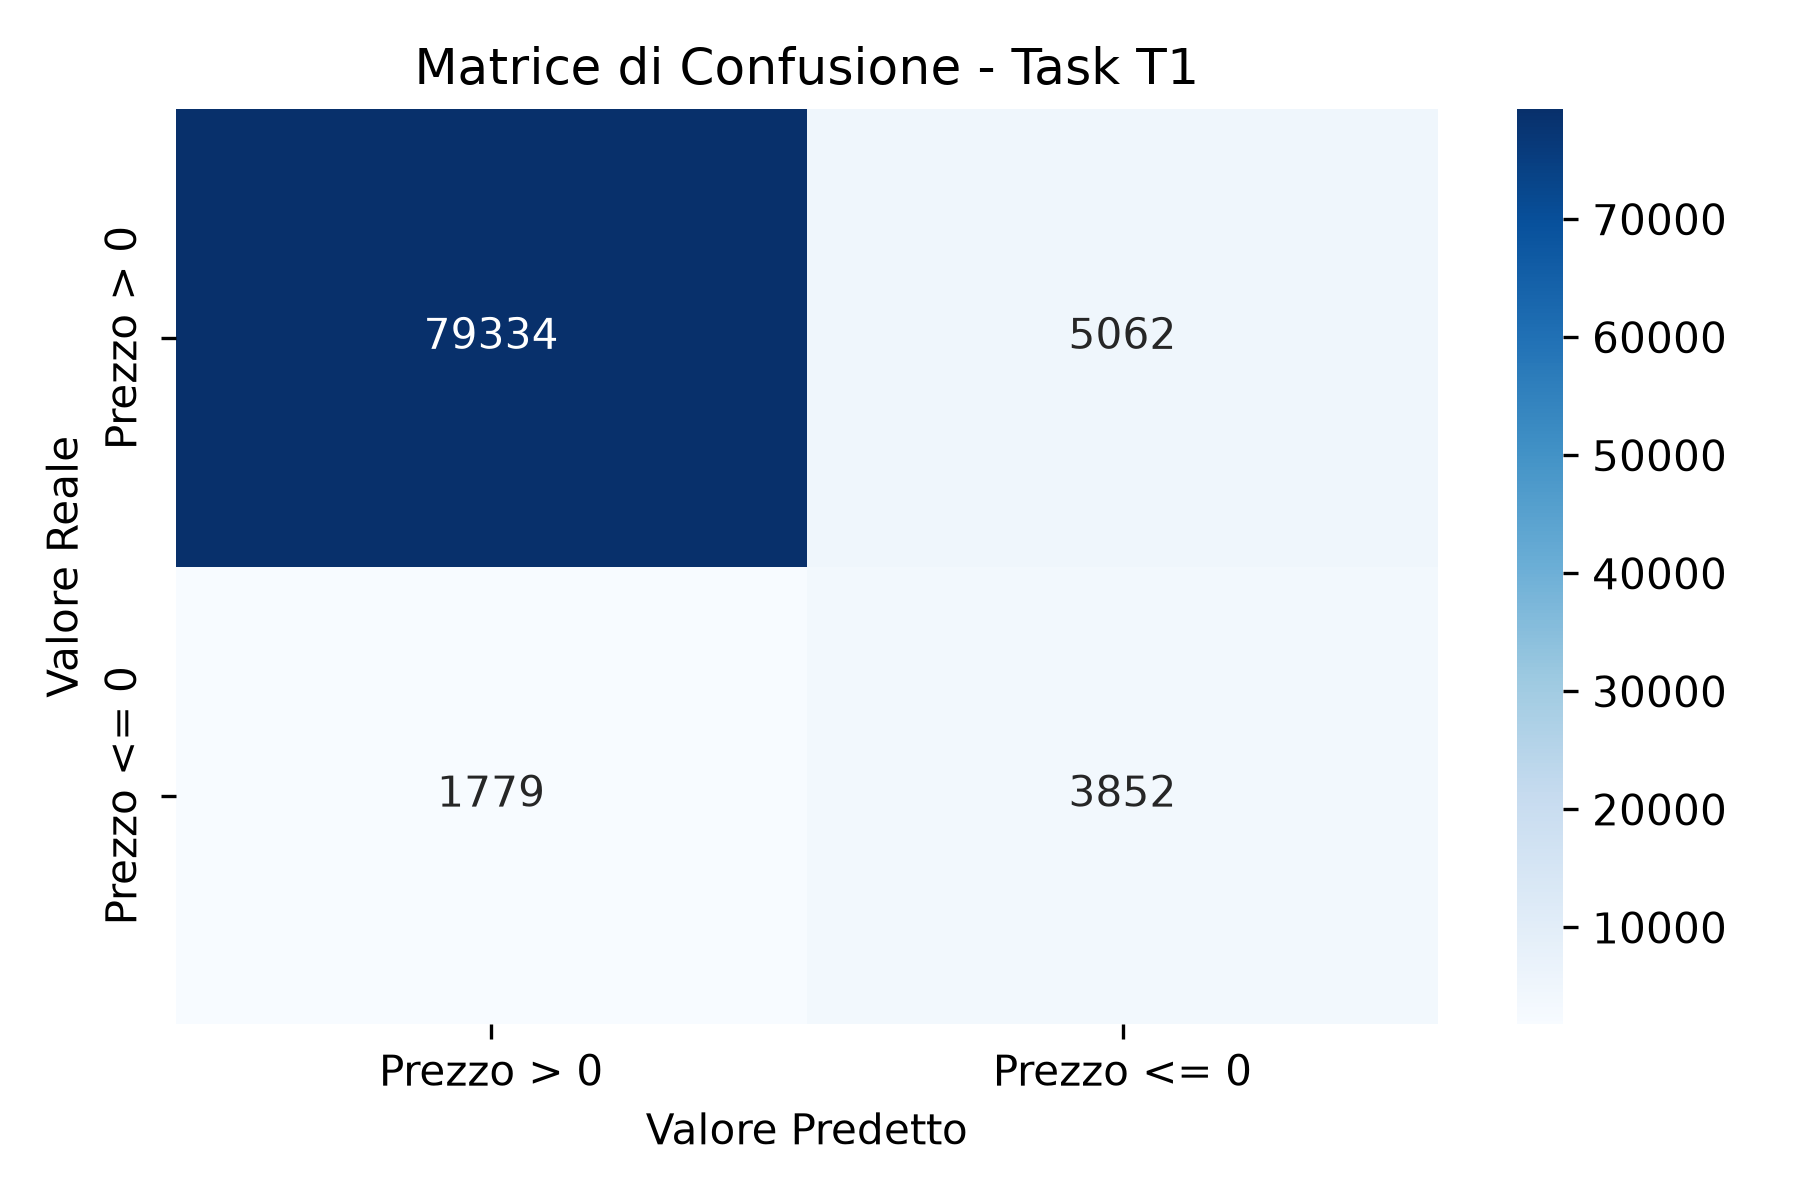
\includegraphics[width=0.5\textwidth]{images/analisi/output/random_forest/matrice_confusione_t1.png}
    \captionof{figure}{Matrice di confusione prodotta dal modello Random Forest}
    \label{fig:Matrice di Confusione}
\end{center}

\begin{figure}[ht!]
    \centering
    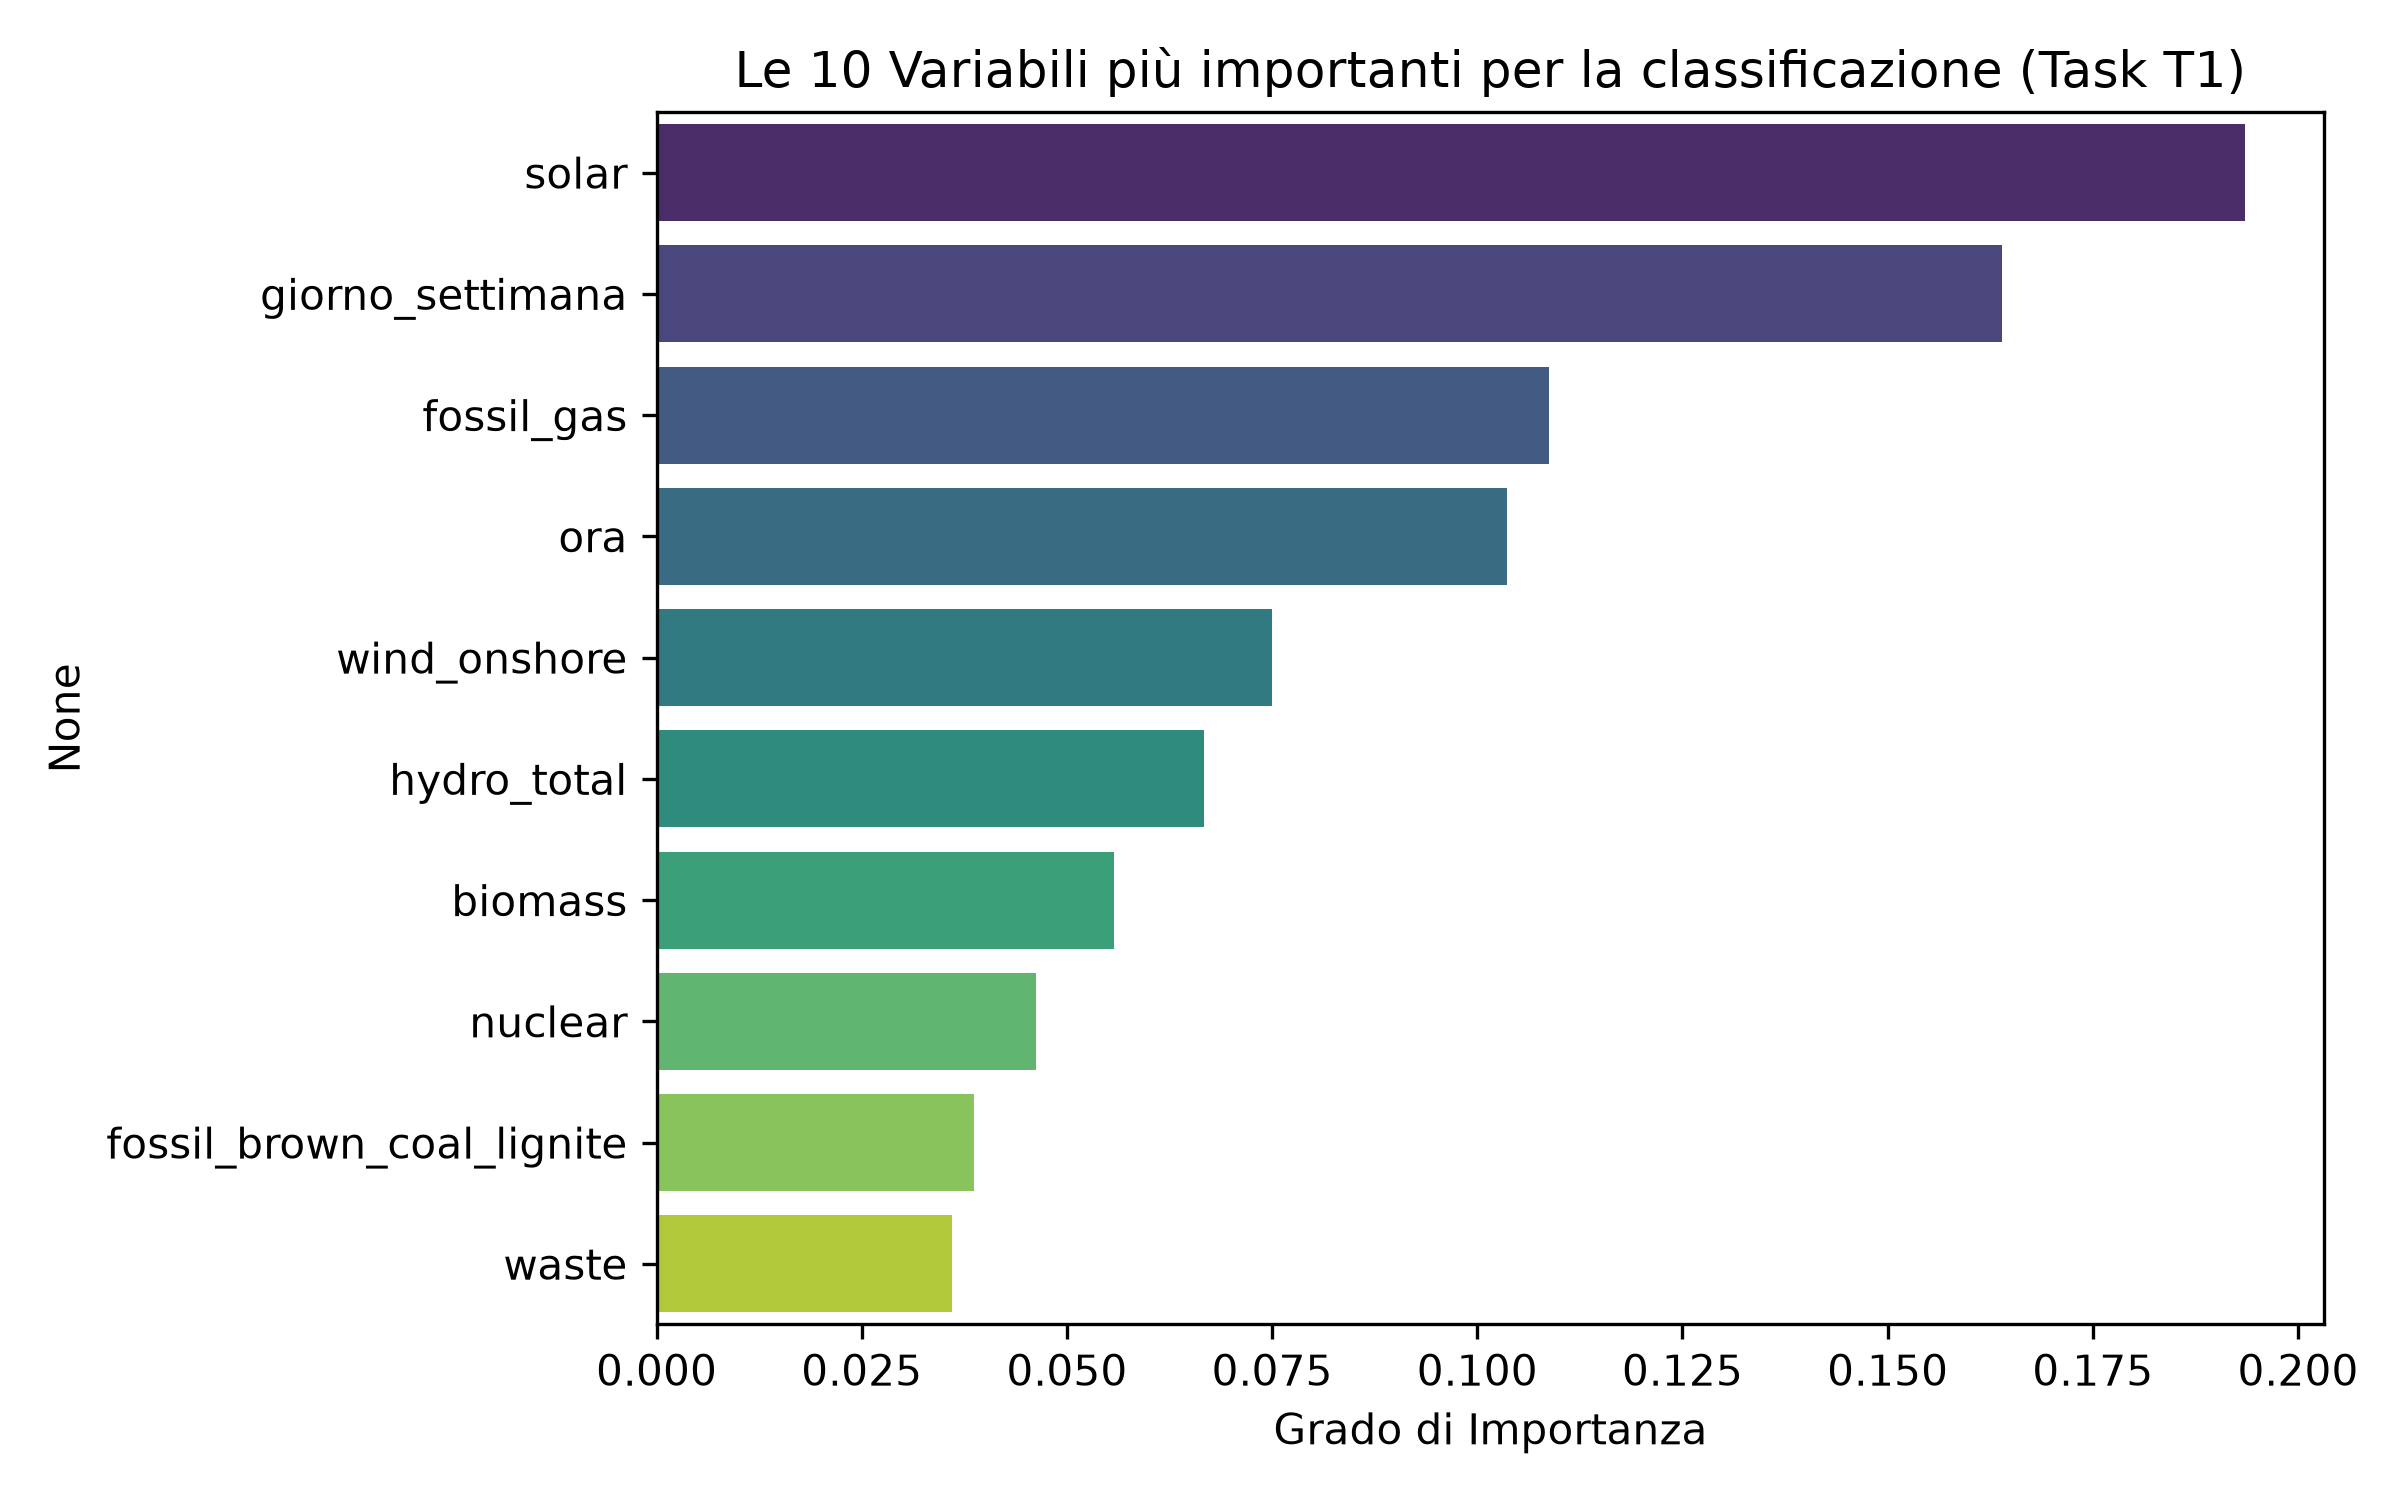
\includegraphics[width=0.8\textwidth]{images/analisi/output/random_forest/feature_importance_t1.png}
    \caption{Le 10 feature più importanti estratte dal modello Random Forest per la classificazione dei prezzi nulli o negativi}
    \label{fig:feature}
\end{figure}

L'algoritmo \textit{Random Forest} è stato selezionato come modello di riferimento per il Task 1 grazie alla sua intrinseca robustezza, alla capacità di gestire relazioni non lineari complesse tra le feature energetiche e temporali, e alla possibilità nativa di bilanciare le classi asimmetriche.

\subsubsection{Miglioramento dell'algoritmo}

Al fine di incrementare l'affidabilità predittiva e ridurre i falsi allarmi senza compromettere la sensibilità del classificatore, è stata condotta un'attività di ottimizzazione iterativa. La configurazione finale ottimizzata ha previsto:
\begin{itemize}
    \item \textbf{\texttt{n\_estimators = 300}:} incremento del numero di alberi per stabilizzare la votazione d'insieme.
    \item \textbf{\texttt{max\_depth = 25}:} innalzamento della profondità massima per consentire l'apprendimento di pattern multifattoriali complessi (es. interazioni tra picchi fotovoltaici e ora del giorno).
    \item \textbf{\texttt{min\_samples\_leaf = 2}:} introduzione di un vincolo sul numero minimo di campioni per foglia per prevenire fenomeni di \textit{overfitting}.
    \item \textbf{\texttt{class\_weight = "balanced\_subsample"}:} ricalcolo dinamico dei pesi di penalizzazione dell'errore per ciascun sottoinsieme di campionamento dei singoli alberi.
\end{itemize}

I risultati ottenuti sul Test Set (dati 2025) con il modello ottimizzato riflettono le dinamiche del partizionamento temporale applicato. Sulla classe minoritaria (Prezzo $\leq$ 0 \euro / MWh) si evidenzia il seguente bilanciamento:
\begin{itemize}
    \item \textbf{Precision:} $69\%$ (il modello risulta altamente affidabile quando genera un allarme, contenendo i falsi positivi a sole 976 istanze su oltre 90.000 osservazioni totali).
    \item \textbf{Recall:} $39\%$ (la capacità di intercettare i crolli reali nel nuovo orizzonte temporale inedito si riduce: il modello sacrifica parte della sensibilità per garantire l'affidabilità delle previsioni effettuate).
    \item \textbf{F1-Score:} $50\%$ (valore di sintesi che riflette il \textit{trade-off} tra l'elevata precisione e la flessione della recall dovuta allo spostamento temporale della distribuzione).
    \item \textbf{Accuracy Globale:} $95\%$.
\end{itemize}

\section{T1: K-Nearest Neighbors (KNN)}

Utilizzando l'algortimo di ML \textit{K-Nearest Neighbors (KNN)} si hanno i seguenti risultati:

\begin{table}[htbp]
    \centering
    \caption{Report di classificazione del KNN (Task 1)}
    \label{tab:report_knn_task1}
    \begin{tabular}{|l|c|c|c|c|}
        \hline
        \textbf{Classe} & \textbf{Precision} & \textbf{Recall} & \textbf{F1-Score} & \textbf{Supporto} \\ \hline
        Prezzo $>$ 0    & 0.96 & 0.99 & 0.97 & 84396 \\ \hline
        Prezzo $\leq$ 0 & 0.65 & 0.39 & 0.49 & 5631 \\ \hline
        \textit{Accuracy}     &      &      & 0.95 & 90027 \\ \hline
        \textit{Macro avg}    & 0.81 & 0.69 & 0.73 & 90027 \\ \hline
        \textit{Weighted avg} & 0.94 & 0.95 & 0.94 & 90027 \\ \hline
    \end{tabular}
\end{table}

Riepilogo delle metriche aggiunte: 

\begin{table}[htbp]
    \centering
    \caption{Metriche aggiuntive del modello KNN (Task 1)}
    \label{tab:metriche_knn_task1}
    \begin{tabular}{|l|c|}
        \hline
        \textbf{Metrica} & \textbf{Valore} \\ \hline
        Accuracy & 0.9491 \\ \hline
        Precision & 0.6541 \\ \hline
        Recall & 0.3950 \\ \hline
        F1-Score & 0.4925 \\ \hline
        ROC-AUC & 0.8266 \\ \hline
        PR-AUC & 0.4378 \\ \hline
    \end{tabular}
\end{table}

\begin{center}
    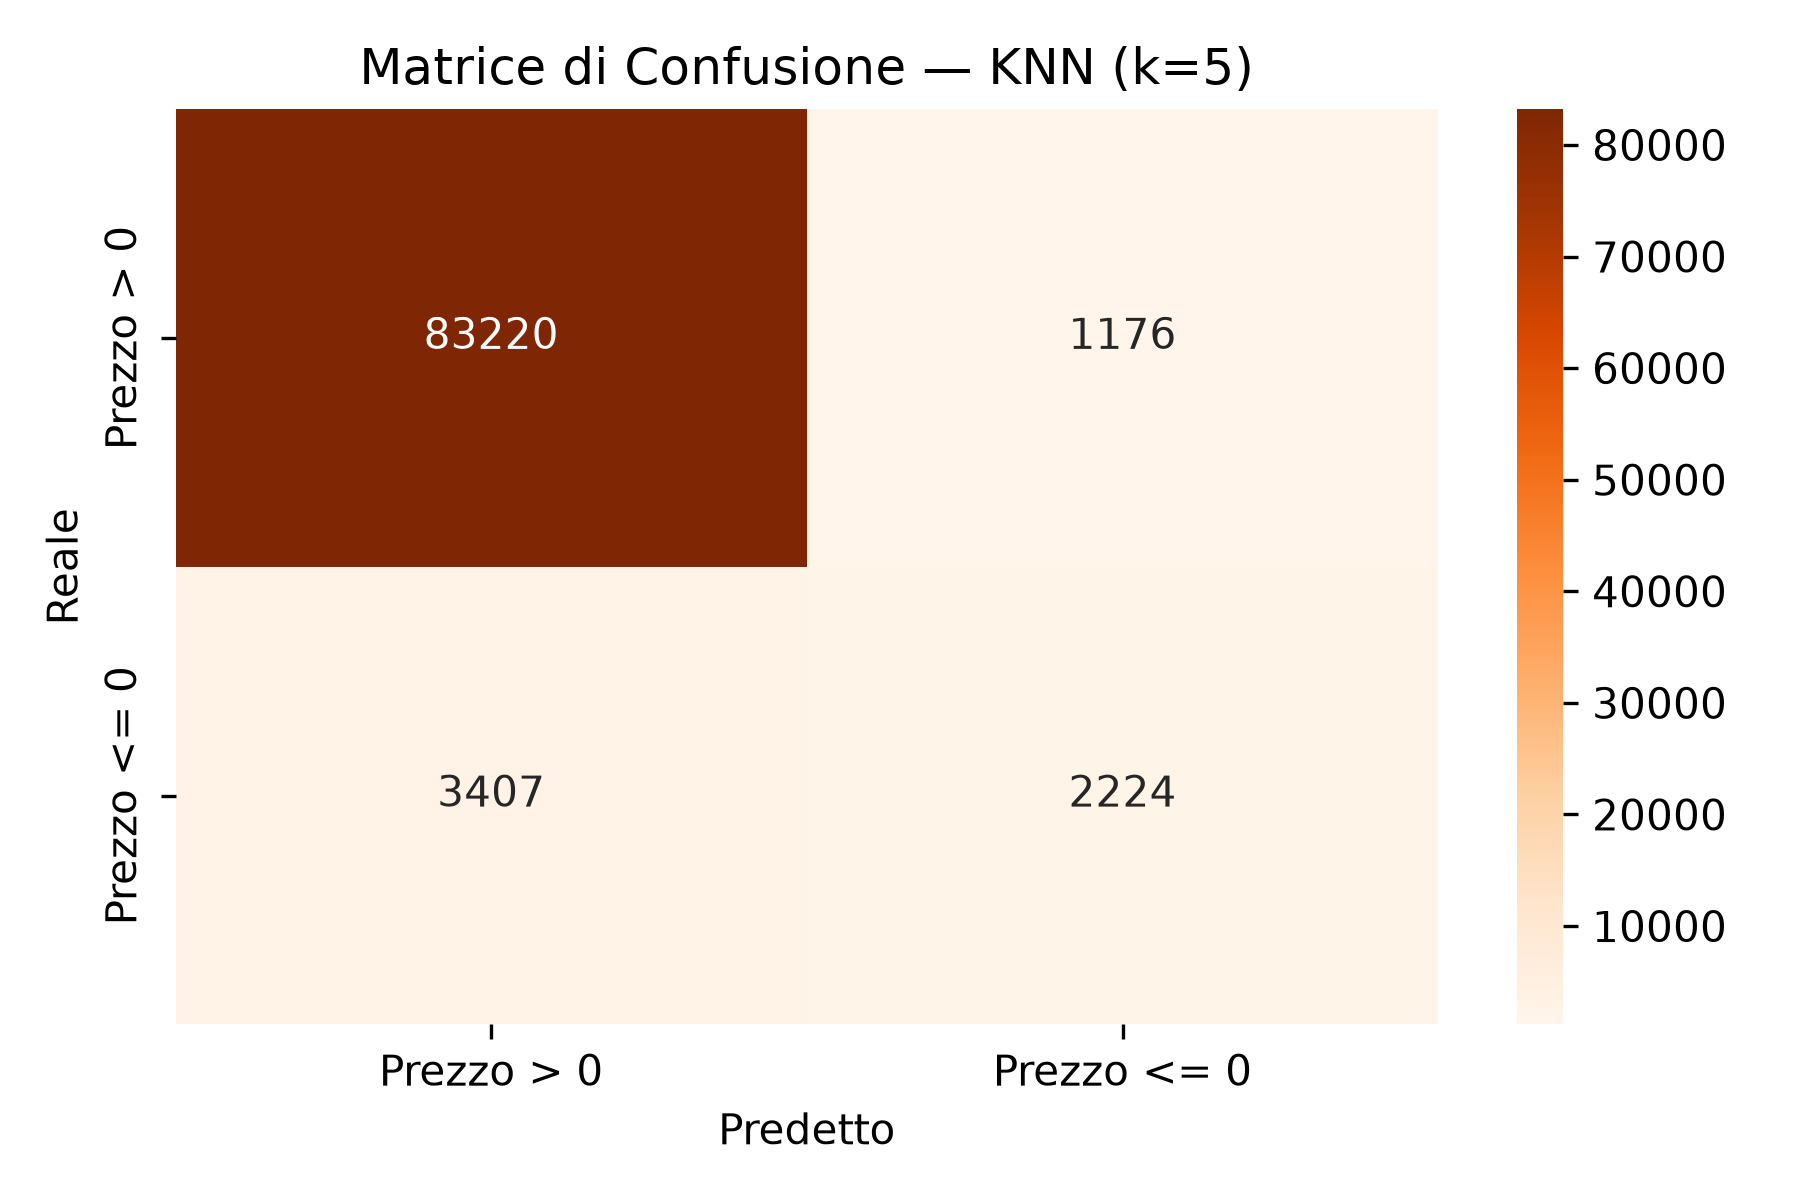
\includegraphics[width=0.8\textwidth]{images/analisi/output/knn/matrice_confusione_knn_t1.png}
    \captionof{figure}{Matrice di confusione prodotta dal modello KNN}
    \label{fig:Matrice di Confusione}
\end{center}

Come secondo algoritmo di riferimento per il Task 1 è stato valutato il classificatore \textbf{K-Nearest Neighbors (KNN)}. A differenza degli alberi di decisione, il KNN è un modello basato sulle istanze e sulle distanze geometriche nello spazio multidimensionale delle feature, risultando particolarmente sensibile alla scala dei dati.
A causa della natura geometrica dell'algoritmo, che calcola la distanza euclidea (o metriche affini) tra le osservazioni, il KNN ha mostrato notevoli difficoltà nella gestione del forte sbilanciamento delle classi (4.8\% di prezzi negativi contro il 95.2\% positivi).

\newpage

\section{T1: Decision Tree}

Utilizzando l'algoritmo \textit{Decision Tree} si hanno i seguenti risultati:

\begin{table}[htbp]
    \centering
    \caption{Report di classificazione del Decision Tree (Task 1)}
    \label{tab:report_dt_task1}
    \begin{tabular}{|l|c|c|c|c|}
        \hline
        \textbf{Classe} & \textbf{Precision} & \textbf{Recall} & \textbf{F1-Score} & \textbf{Supporto} \\ \hline
        Prezzo $>$ 0    & 0.97 & 0.94 & 0.96 & 84396 \\ \hline
        Prezzo $\leq$ 0 & 0.42 & 0.62 & 0.50 & 5631 \\ \hline
        \textit{Accuracy}     &      &      & 0.92 & 90027 \\ \hline
        \textit{Macro avg}    & 0.70 & 0.78 & 0.73 & 90027 \\ \hline
        \textit{Weighted avg} & 0.94 & 0.92 & 0.93 & 90027 \\ \hline
    \end{tabular}
\end{table}

\begin{figure}[ht!]
    \centering
    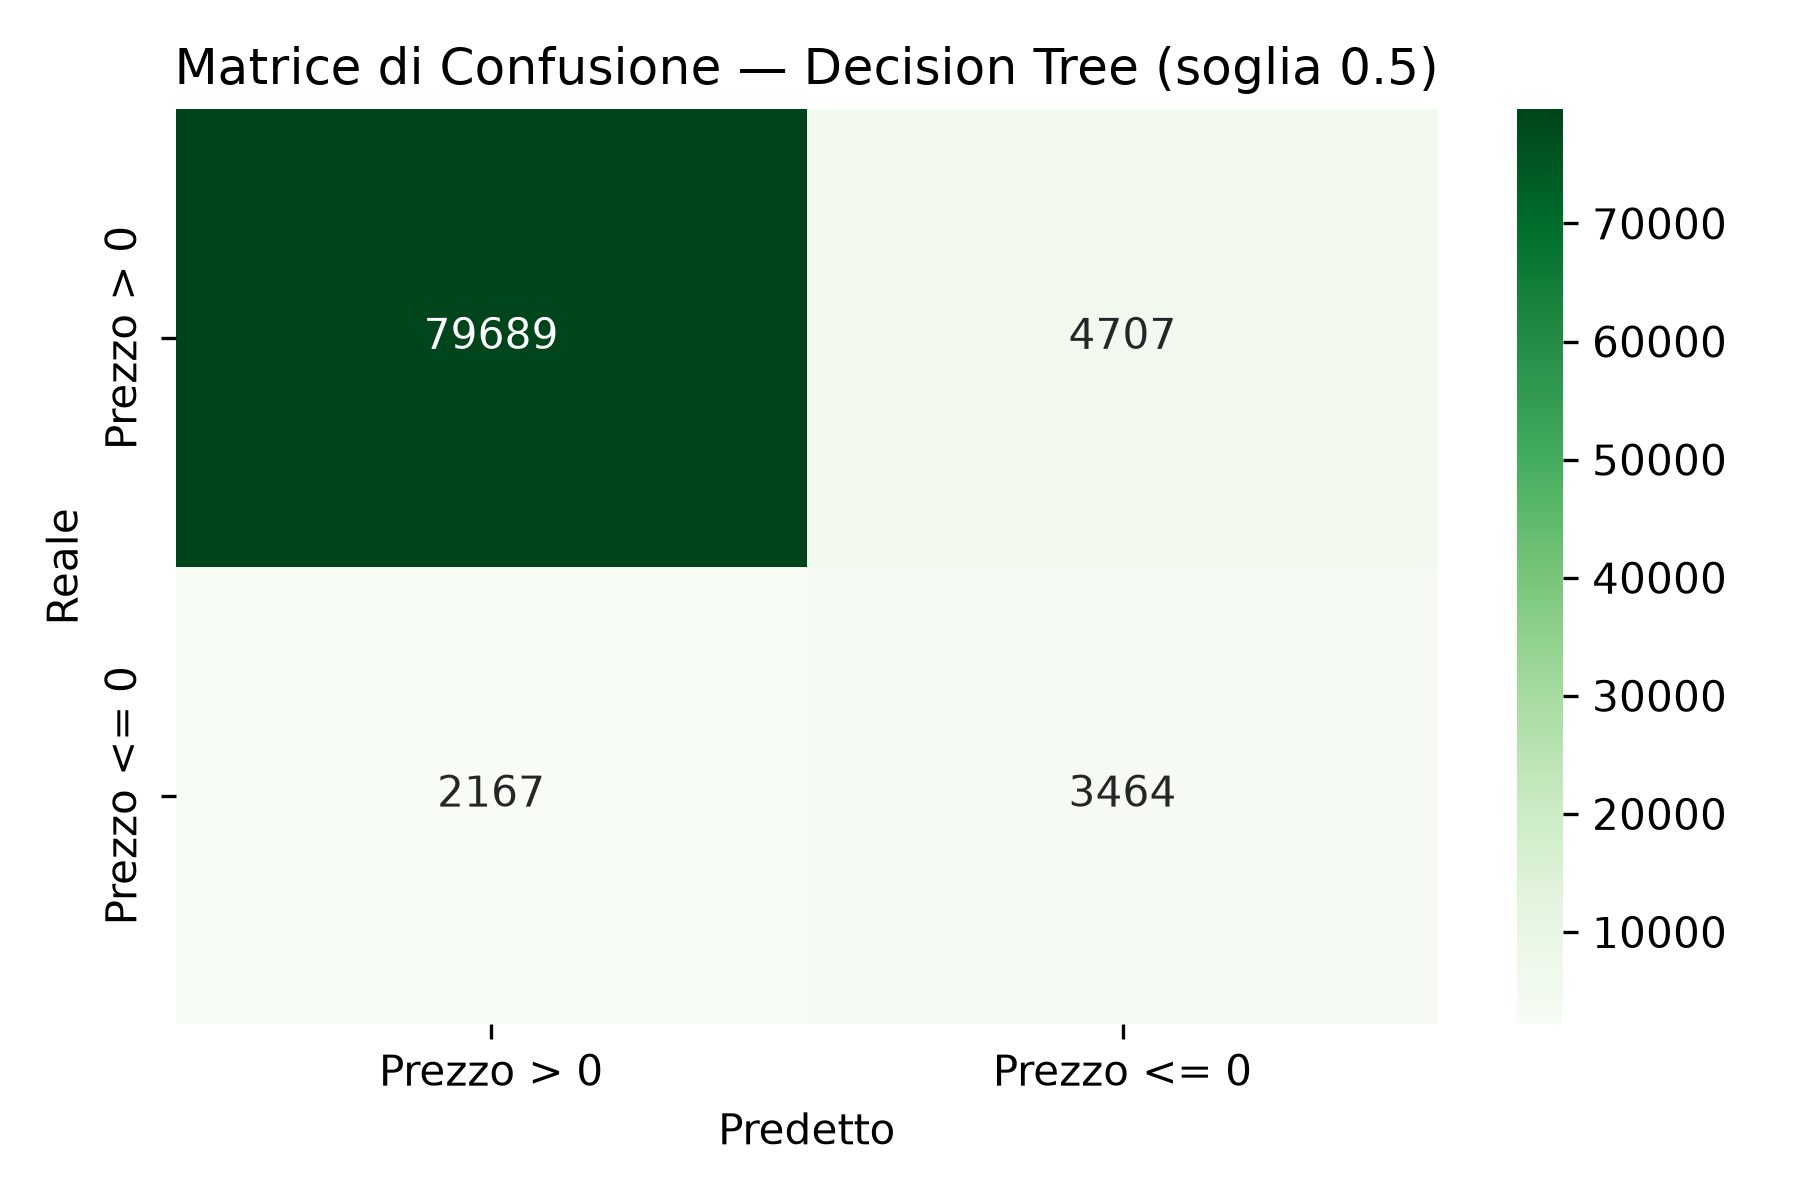
\includegraphics[width=0.8\textwidth]{images/analisi/output/decision_tree/matrice_confusione_dt_t1.png}
    \caption{Matrice di confusione Decision Tree}
    \label{fig:Decision Tree}
\end{figure}

Come terzo modello analizzato per il Task 1 è stato valutato l'algoritmo del \textbf{Decision Tree (Albero di Decisione)}. A differenza del \textit{Random Forest}, che si basa su una foresta di alberi decorrelati, il Decision Tree costruisce un'unica struttura gerarchica di regole di decisione basate sulla suddivisione ricorsiva dello spazio delle feature (\textit{recursive splitting}).

Tuttavia, applicato al dataset che è fortemente sbilanciato, il Decision Tree singolo ha evidenziato notevoli limiti di stabilità:
\begin{itemize}
    \item \textbf{Tendenza all'Overfitting:} Senza un rigoroso controllo della profondità massima o dei campioni minimi per foglia, il singolo albero tende a memorizzare le particolarità del Training Set, perdendo capacità di generalizzazione sul Test Set.
    \item \textbf{Varianza Elevata:} Piccole variazioni nei dati di addestramento possono alterare radicalmente la struttura dell'albero e le soglie di taglio, risultando in performance meno robuste.
\end{itemize}

\newpage

\section{T1: Naive Bayes}

Utilizzando l'algoritmo \textit{Naive Bayes} si hanno i seguenti risultati:

\begin{table}[htbp]
\centering
\caption{Report di classificazione del modello Naive Bayes per il Task 1}
\label{tab:naive_bayes_task1}
\begin{tabular}{|l|c|c|c|c|}
\hline
\textbf{Classe} & \textbf{Precision} & \textbf{Recall} & \textbf{F1-score} & \textbf{Support} \\
\hline
Prezzo $> 0$ & 0.96 & 0.96 & 0.96 & 84396 \\
\hline
Prezzo $\leq 0$ & 0.37 & 0.36 & 0.36 & 5631 \\
\hline
Accuracy & -- & -- & 0.92 & 90027 \\
\hline
Macro avg & 0.67 & 0.66 & 0.66 & 90027 \\
\hline
Weighted avg & 0.92 & 0.92 & 0.92 & 90027 \\
\hline
\end{tabular}
\end{table}

\begin{figure}[ht!]
    \centering
    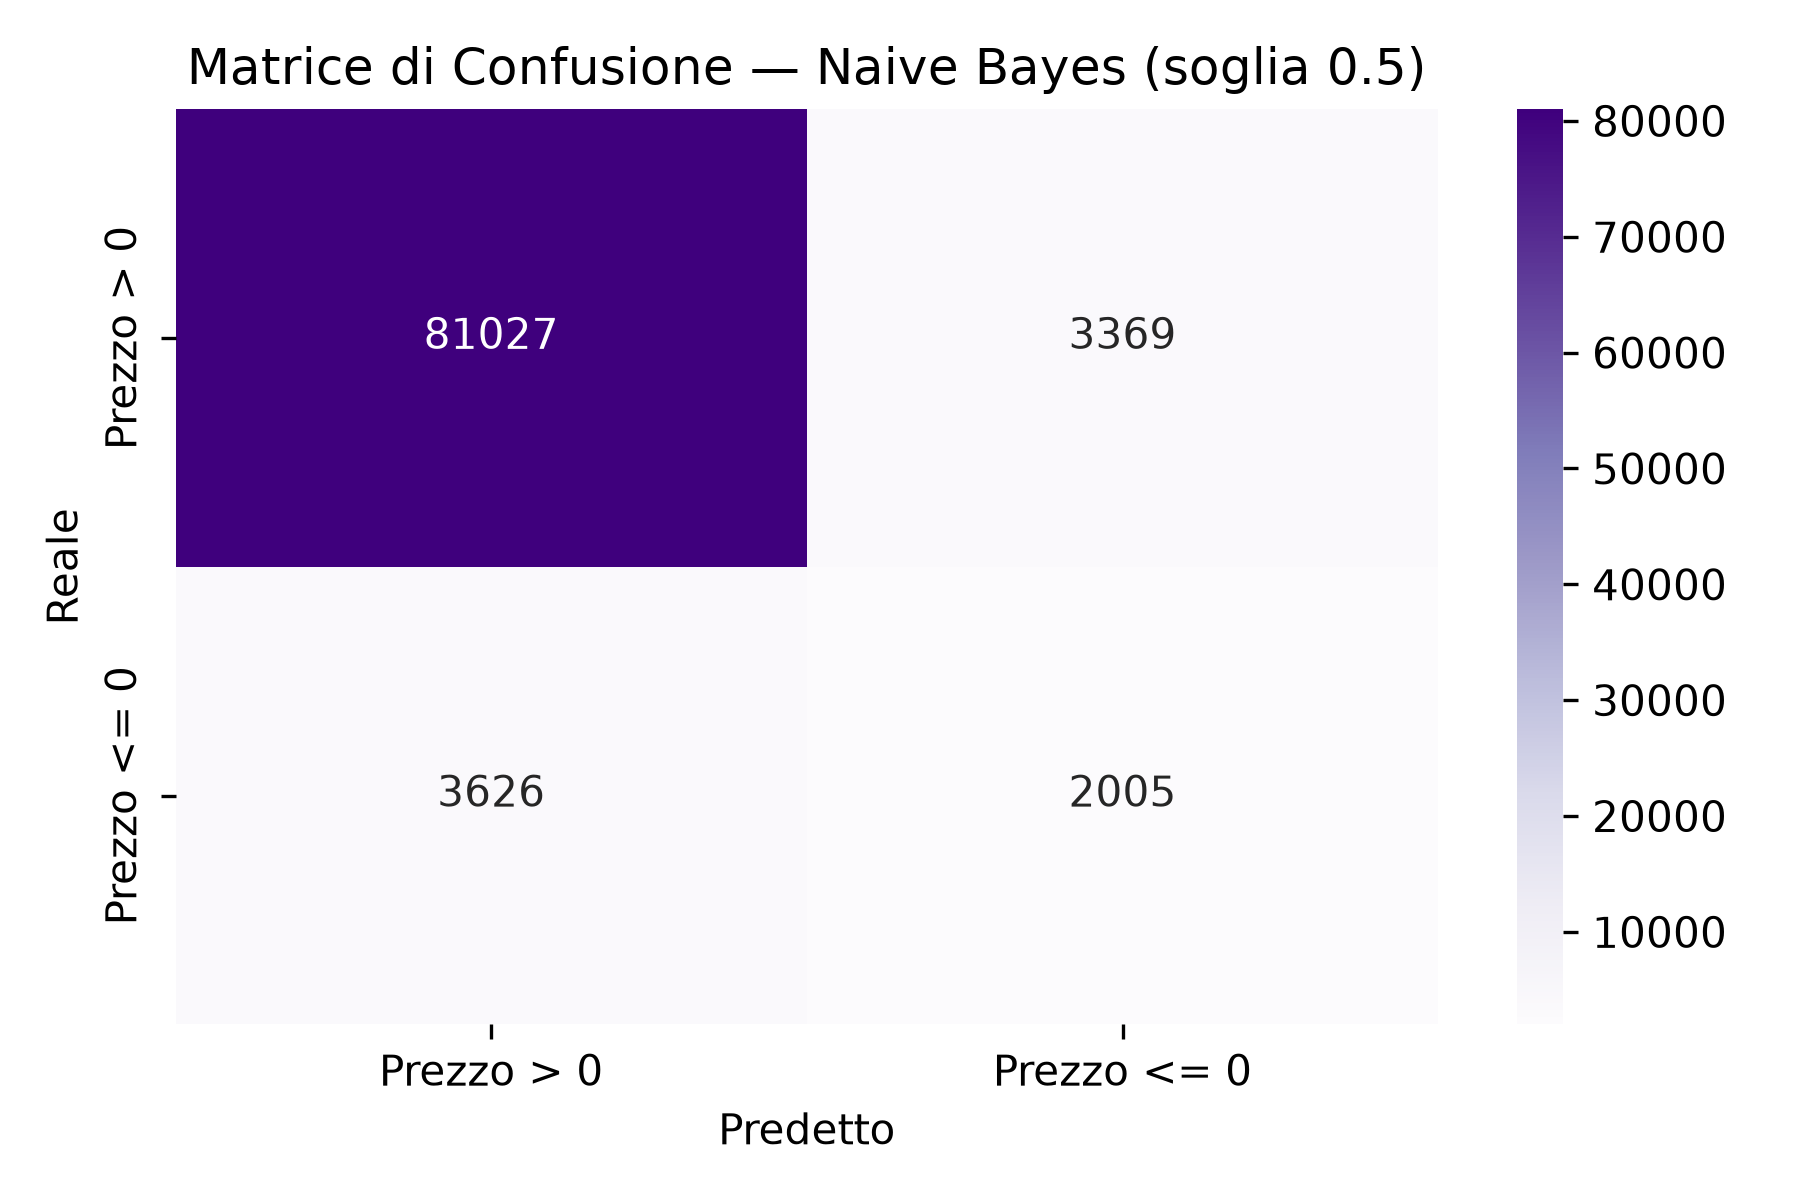
\includegraphics[width=0.8\textwidth]{images/analisi/output/naive_bayes/matrice_confusione_nb_t1.png}
    \caption{Matrice di confusione Naive Bayes}
    \label{fig:Naive Bayes}
\end{figure}

Il principale vantaggio del Naive Bayes risiede nella sua estrema efficienza computazionale e nella rapidità di addestramento. Tuttavia, nel contesto specifico della previsione dei prezzi dell'energia elettrica basata su volumi di generazione e variabili temporali, il modello mostra limiti strutturali evidenti:
\begin{itemize}
    \item \textbf{L'ipotesi di indipendenza:} L'assunzione che le feature (es. la produzione solare e quella eolica, o l'ora del giorno) siano statisticamente indipendenti tra loro è fortemente violata nei mercati energetici. Le fonti rinnovabili e i profili di carico seguono dinamiche fisiche e temporali profondamente correlate.
\end{itemize}

\newpage

\section{T1: Gradient Boosting}
\label{sec:t1_gradient_boosting}

Utilizzando l'algoritmo \textit{Gradient Boosting} si hanno i seguenti risultati:

\begin{table}[htbp]
    \centering
    \caption{Report di classificazione del Gradient Boosting (Task 1)}
    \label{tab:report_gb_task1}
    \begin{tabular}{|l|c|c|c|c|}
        \hline
        \textbf{Classe} & \textbf{Precision} & \textbf{Recall} & \textbf{F1-Score} & \textbf{Supporto} \\ \hline
        Prezzo $>$ 0    & 0.97 & 0.99 & 0.98 & 84396 \\ \hline
        Prezzo $\leq$ 0 & 0.74 & 0.31 & 0.43 & 5631  \\ \hline
        \textit{Accuracy}     & \multicolumn{2}{c|}{} & 0.96 & 90027 \\ \hline
        \textit{Macro avg}    & 0.86 & 0.65 & 0.71 & 90027 \\ \hline
        \textit{Weighted avg} & 0.95 & 0.96 & 0.95 & 90027 \\ \hline
    \end{tabular}
\end{table}

\begin{figure}[htbp]
    \centering
    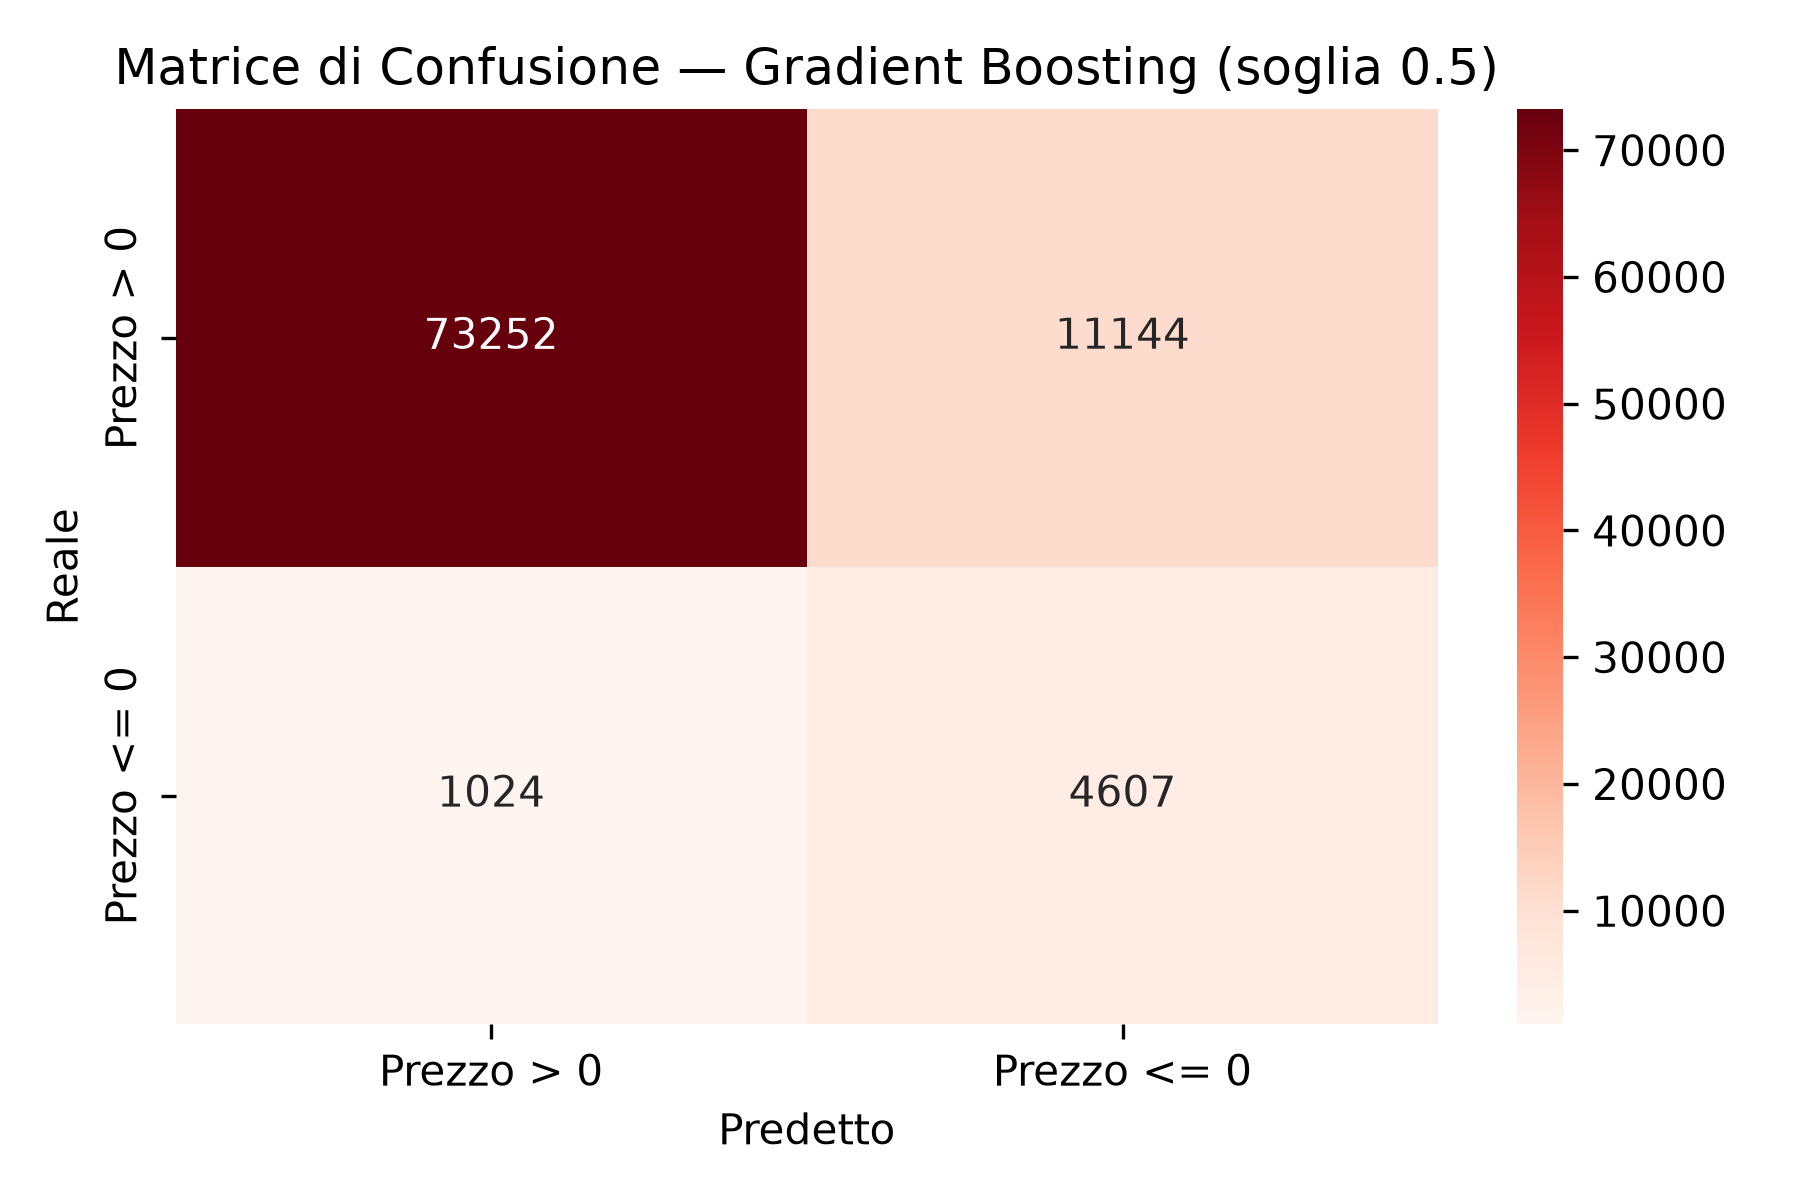
\includegraphics[width=0.8\textwidth]{images/analisi/output/gradient_boosting/matrice_confusione_gb_t1.png}
    \caption{Matrice di confusione prodotta dal modello Gradient Boosting (Test Set 2025).}
    \label{fig:matrice_confusione_gb}
\end{figure}


Il quinto algoritmo analizzato per il Task 1 è il \textbf{Gradient Boosting}, un modello di \textit{ensemble} basato sul boosting sequenziale di alberi decisionali deboli (\textit{weak learners}). L'algoritmo costruisce iterativamente gli alberi in modo tale che ciascun nuovo albero corregga gli errori residui commessi dai precedenti, minimizzando una funzione di perdita differenziabile.

Nel contesto del Task 1, il Gradient Boosting standard non dispone di un parametro nativo \texttt{class\_weight}. Per colmare questa lacuna e gestire il forte sbilanciamento delle classi, in fase di addestramento è stata applicata una penalizzazione esplicita tramite vettori di pesi (\textit{sample weights}), assegnando un peso maggiore agli errori commessi sulla classe minoritaria dei prezzi negativi. 

I risultati evidenziano un'elevata \textit{Precision} ($74\%$), segno che il modello è molto affidabile quando prevede un crollo di prezzo, affiancata tuttavia da una \textit{Recall} contenuta ($31\%$), confermando la necessità di valutare ulteriori strategie di bilanciamento (quali l'oversampling) descritte nella sezione successiva.

\section{T1: Gradient Boosting con Ottimizzazione della Soglia}
\label{sec:t1_gradient_boosting_soglia}

Sebbene l'utilizzo dei pesi correttivi (\textit{sample weights}) abbia permesso al \textit{Gradient Boosting} di intercettare i crolli di prezzo, l'adozione della soglia di classificazione standard ($p = 0.5$) genera un eccesso di falsi positivi. Per massimizzare l'equilibrio predittivo senza alterare l'addestramento, si è proceduto all'ottimizzazione della soglia decisionale tramite una procedura di validazione interna (\textit{Hold-Out} stratificato all'interno del Training Set, evitando rigorosamente qualsiasi \textit{data leakage} sul Test Set).

Analizzando la curva Precision-Recall sul set di validazione, è stata individuata la soglia ottimale di probabilità pari a \textbf{0.82}, calibrata per massimizzare l'F1-Score sulla classe minoritaria.

\begin{table}[htbp]
    \centering
    \caption{Report di classificazione del Gradient Boosting con soglia ottimizzata a 0.82 (Task 1)}
    \label{tab:report_gb_soglia_task1}
    \begin{tabular}{|l|c|c|c|c|}
        \hline
        \textbf{Classe} & \textbf{Precision} & \textbf{Recall} & \textbf{F1-Score} & \textbf{Supporto} \\ \hline
        Prezzo $>$ 0    & 0.97 & 0.98 & 0.97 & 84396 \\ \hline
        Prezzo $\leq$ 0 & 0.58 & 0.51 & 0.54 & 5631  \\ \hline
        \textit{Accuracy}     & \multicolumn{2}{c|}{} & 0.95 & 90027 \\ \hline
        \textit{Macro avg}    & 0.77 & 0.74 & 0.76 & 90027 \\ \hline
        \textit{Weighted avg} & 0.94 & 0.95 & 0.94 & 90027 \\ \hline
    \end{tabular}
\end{table}

\begin{figure}[htbp]
    \centering
    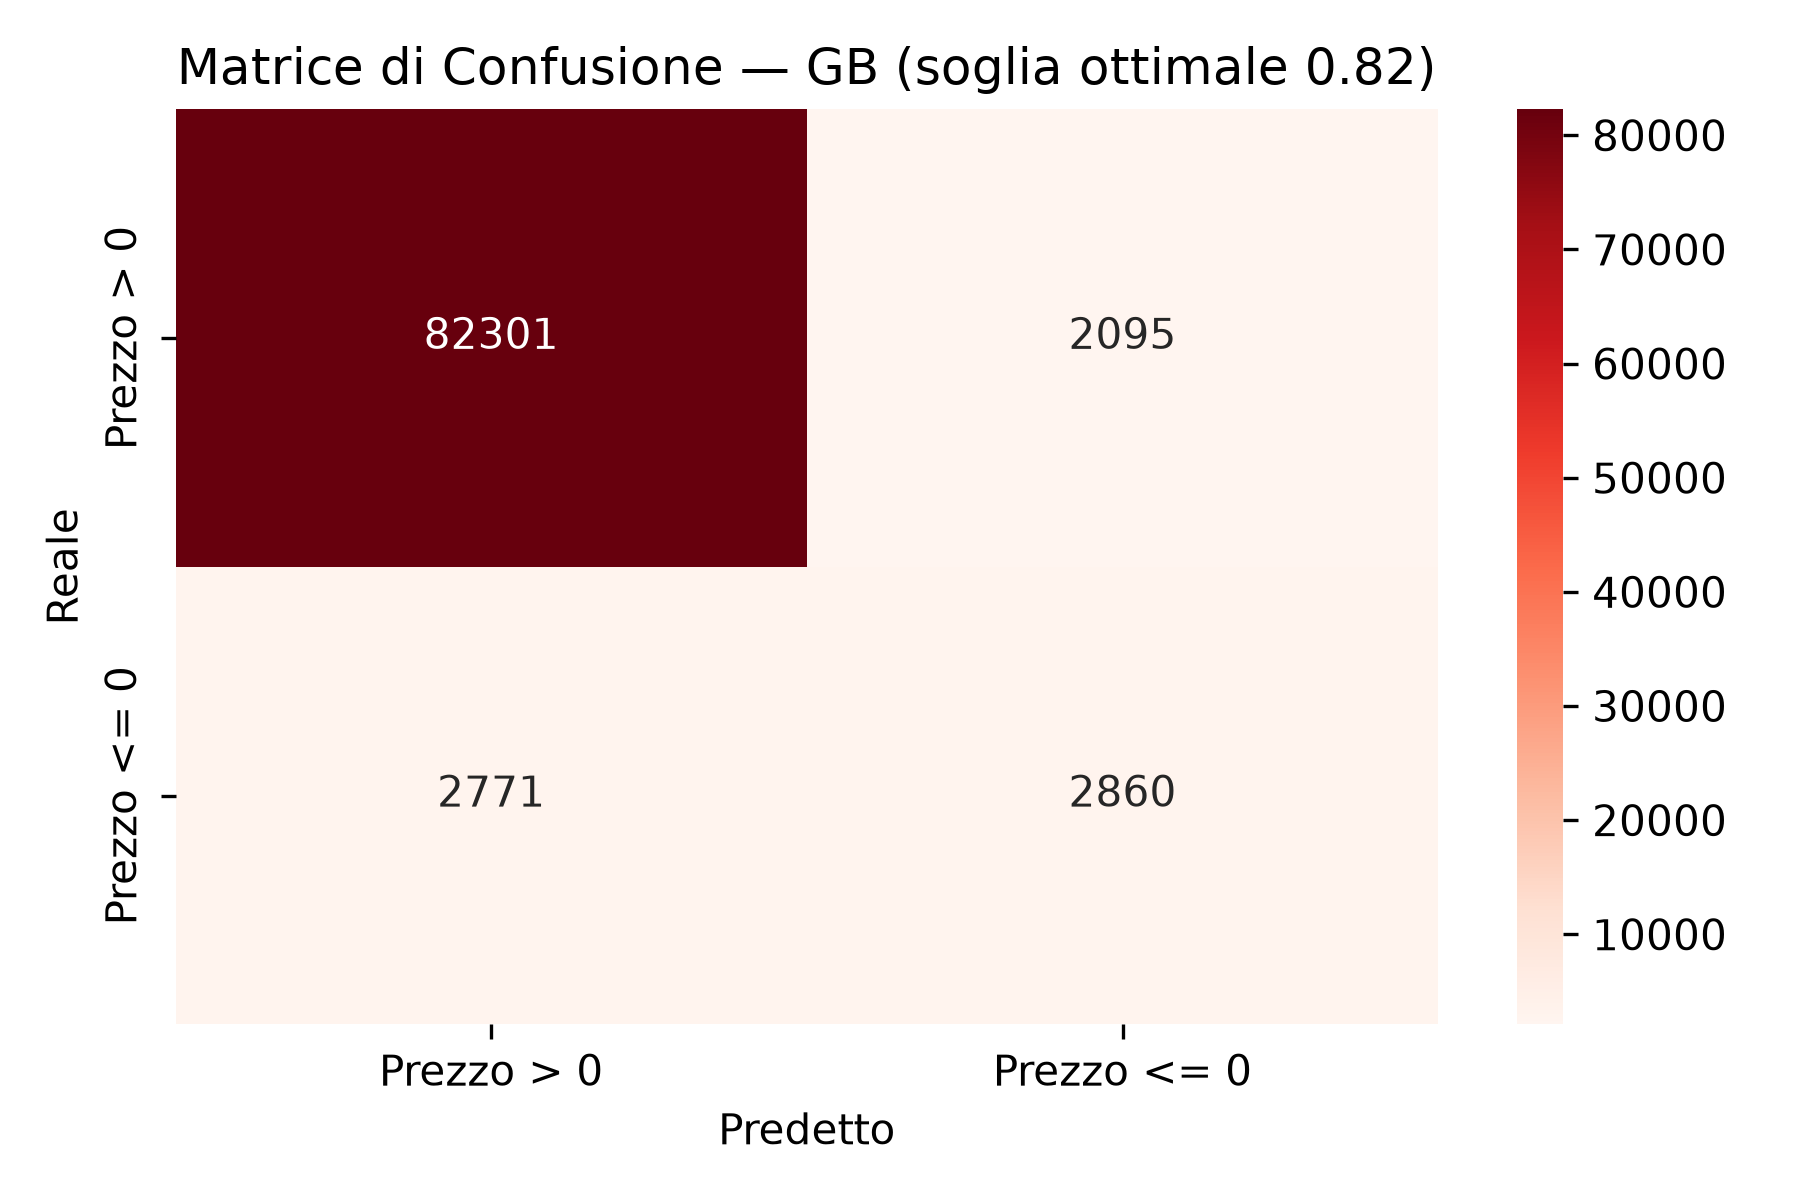
\includegraphics[width=0.6\textwidth]{images/analisi/output/gradient_boosting/matrice_confusione_gb_soglia_0.82.png}
    \caption{Matrice di confusione del Gradient Boosting con soglia decisionale ottimizzata ($\tau = 0.82$).}
    \label{fig:matrice_confusione_gb_soglia}
\end{figure}

L'applicazione della soglia di 0.82 sul Test Set del 2025 ha prodotto un netto miglioramento complessivo:
\begin{itemize}
    \item \textbf{Precision ($58\%$):} Raddoppiata rispetto alla configurazione di base, con un forte abbattimento dei falsi allarmi.
    \item \textbf{Recall ($51\%$):} Mantenuta su livelli stabili e superiori al cinquanta percento dei crolli reali intercettati.
    \item \textbf{F1-Score ($54\%$):} Incrementato di oltre 11 punti percentuali, a conferma dell'efficacia della calibrazione a soglia variabile sui modelli di boosting.
\end{itemize}


\subsection{Conclusione e Tabella Comparativa del Task 1}

L'analisi condotta sui classificatori per il Task 1 evidenzia i seguenti risultati riassunti nella tabella~\ref{tab:comparativa_task1}, riassumendo le prestazioni dei modelli valutati per il Task 1, ordinati dal migliore al peggiore in base all'efficacia complessiva sulla classe critica dei prezzi nulli o negativi:

\begin{table}[htbp]
    \centering
    \caption{Tabella comparativa dei modelli per il Task 1 (dal migliore al peggiore).}
    \label{tab:comparativa_task1}
    \begin{tabular}{|l|c|c|c|}
        \hline
        \textbf{Modello} & \textbf{Precision} & \textbf{Recall} & \textbf{F1-Score} \\ \hline
        1. Random Forest Ottimizzato & 69\% & 39\% & 50\% \\ \hline
        2. Gradient Boosting (Soglia Ott.) & 58\% & 51\% & 54\% \\ \hline
        3. K-Nearest Neighbors (KNN) & 65\% & 39\% & 49\% \\ \hline
        4. Decision Tree (Singolo) & 42\% & 62\% & 50\% \\ \hline
        5. Naive Bayes & 37\% & 36\% & 36\% \\ \hline
    \end{tabular}
\end{table}